%!TEX root = paper.tex
\subsection{Cloud Masking ({\tt cloud-mask})}

%\TODO{classification at the image level}

Sea and land surface temperatures (SST and LST), have a significant
influence on the Earth's weather, and as such, estimation of SST from space-borne sensors, such as satellites, is crucial for a
number of applications in environmental sciences. Satellites are often
equipped with special sensors for this purpose, such as the Sea and Land
Surface Temperature Radiometer (SLSTR) on board the Sentinel-3 satellite. In principle, it is possible to make direct measurements of surface
temperature from these satellites everywhere, except when clouds are
present. Clouds can really affect the signals measured by satellites. making it  much harder to retrieve the temperature measurements. One of
the aspects that underpins the derivation of SST is cloud screening,
which is a step that marks each pixel of thousands of satellite images
as containing cloud or clear sky. This has been, historically, performed using either thresholding or Bayesian method. The purpose of this benchmark is to perform this using machine learning.  An example input and output images are given in Figure~\ref{fig:cm-example}. We also summarize the key features of this benchmark in Table~\ref{tab:cloudmask-seg}. Details around objective of the benchmark, description of relevant datasets, and reference implementation are given below.




\begin{small}
\begin{table}
\caption{Summary of the {\tt cloud-mask} Benchmark.}
\label{tab:cloudmask-seg}
\begin{tabular}{p{0.4\columnwidth}p{0.6\columnwidth}}
\hline
%\textbf{CloudMasking} &  \textbf{Features} \\
\hline
{\bf Description} &
Image classification at pixel level of satellite imagery.
\\
\hline
{\bf Objective} &
Classification of pixels of satellite images into cloud and clear sky categories using machine learning.
\\
\hline
{\bf Challenge Stream} & Image Segmentation\\
\hline
{\bf Domain} & Atmospheric Sciences\\
\hline
{\bf Metrics} &  Classification accuracy\\
\hline
{\bf Data} & Type: Images  ($[2400\times3000\times6]$ and $[1200\times1500\times3]$) \\
& Size: 180~GB \\
& Source: CEDA \\
& Location: STFC Servers~\cite{sciml-bench:2021}\\
\hline
{\bf Reference implementation} & SciML-Bench Cloudmask Benchmark~\cite{cloudmask-implementation} \\
\hline
\hline
\end{tabular}
\end{table}
\end{small}

%\FloatBarrier

\begin{figure}[!htb]
    \centering
    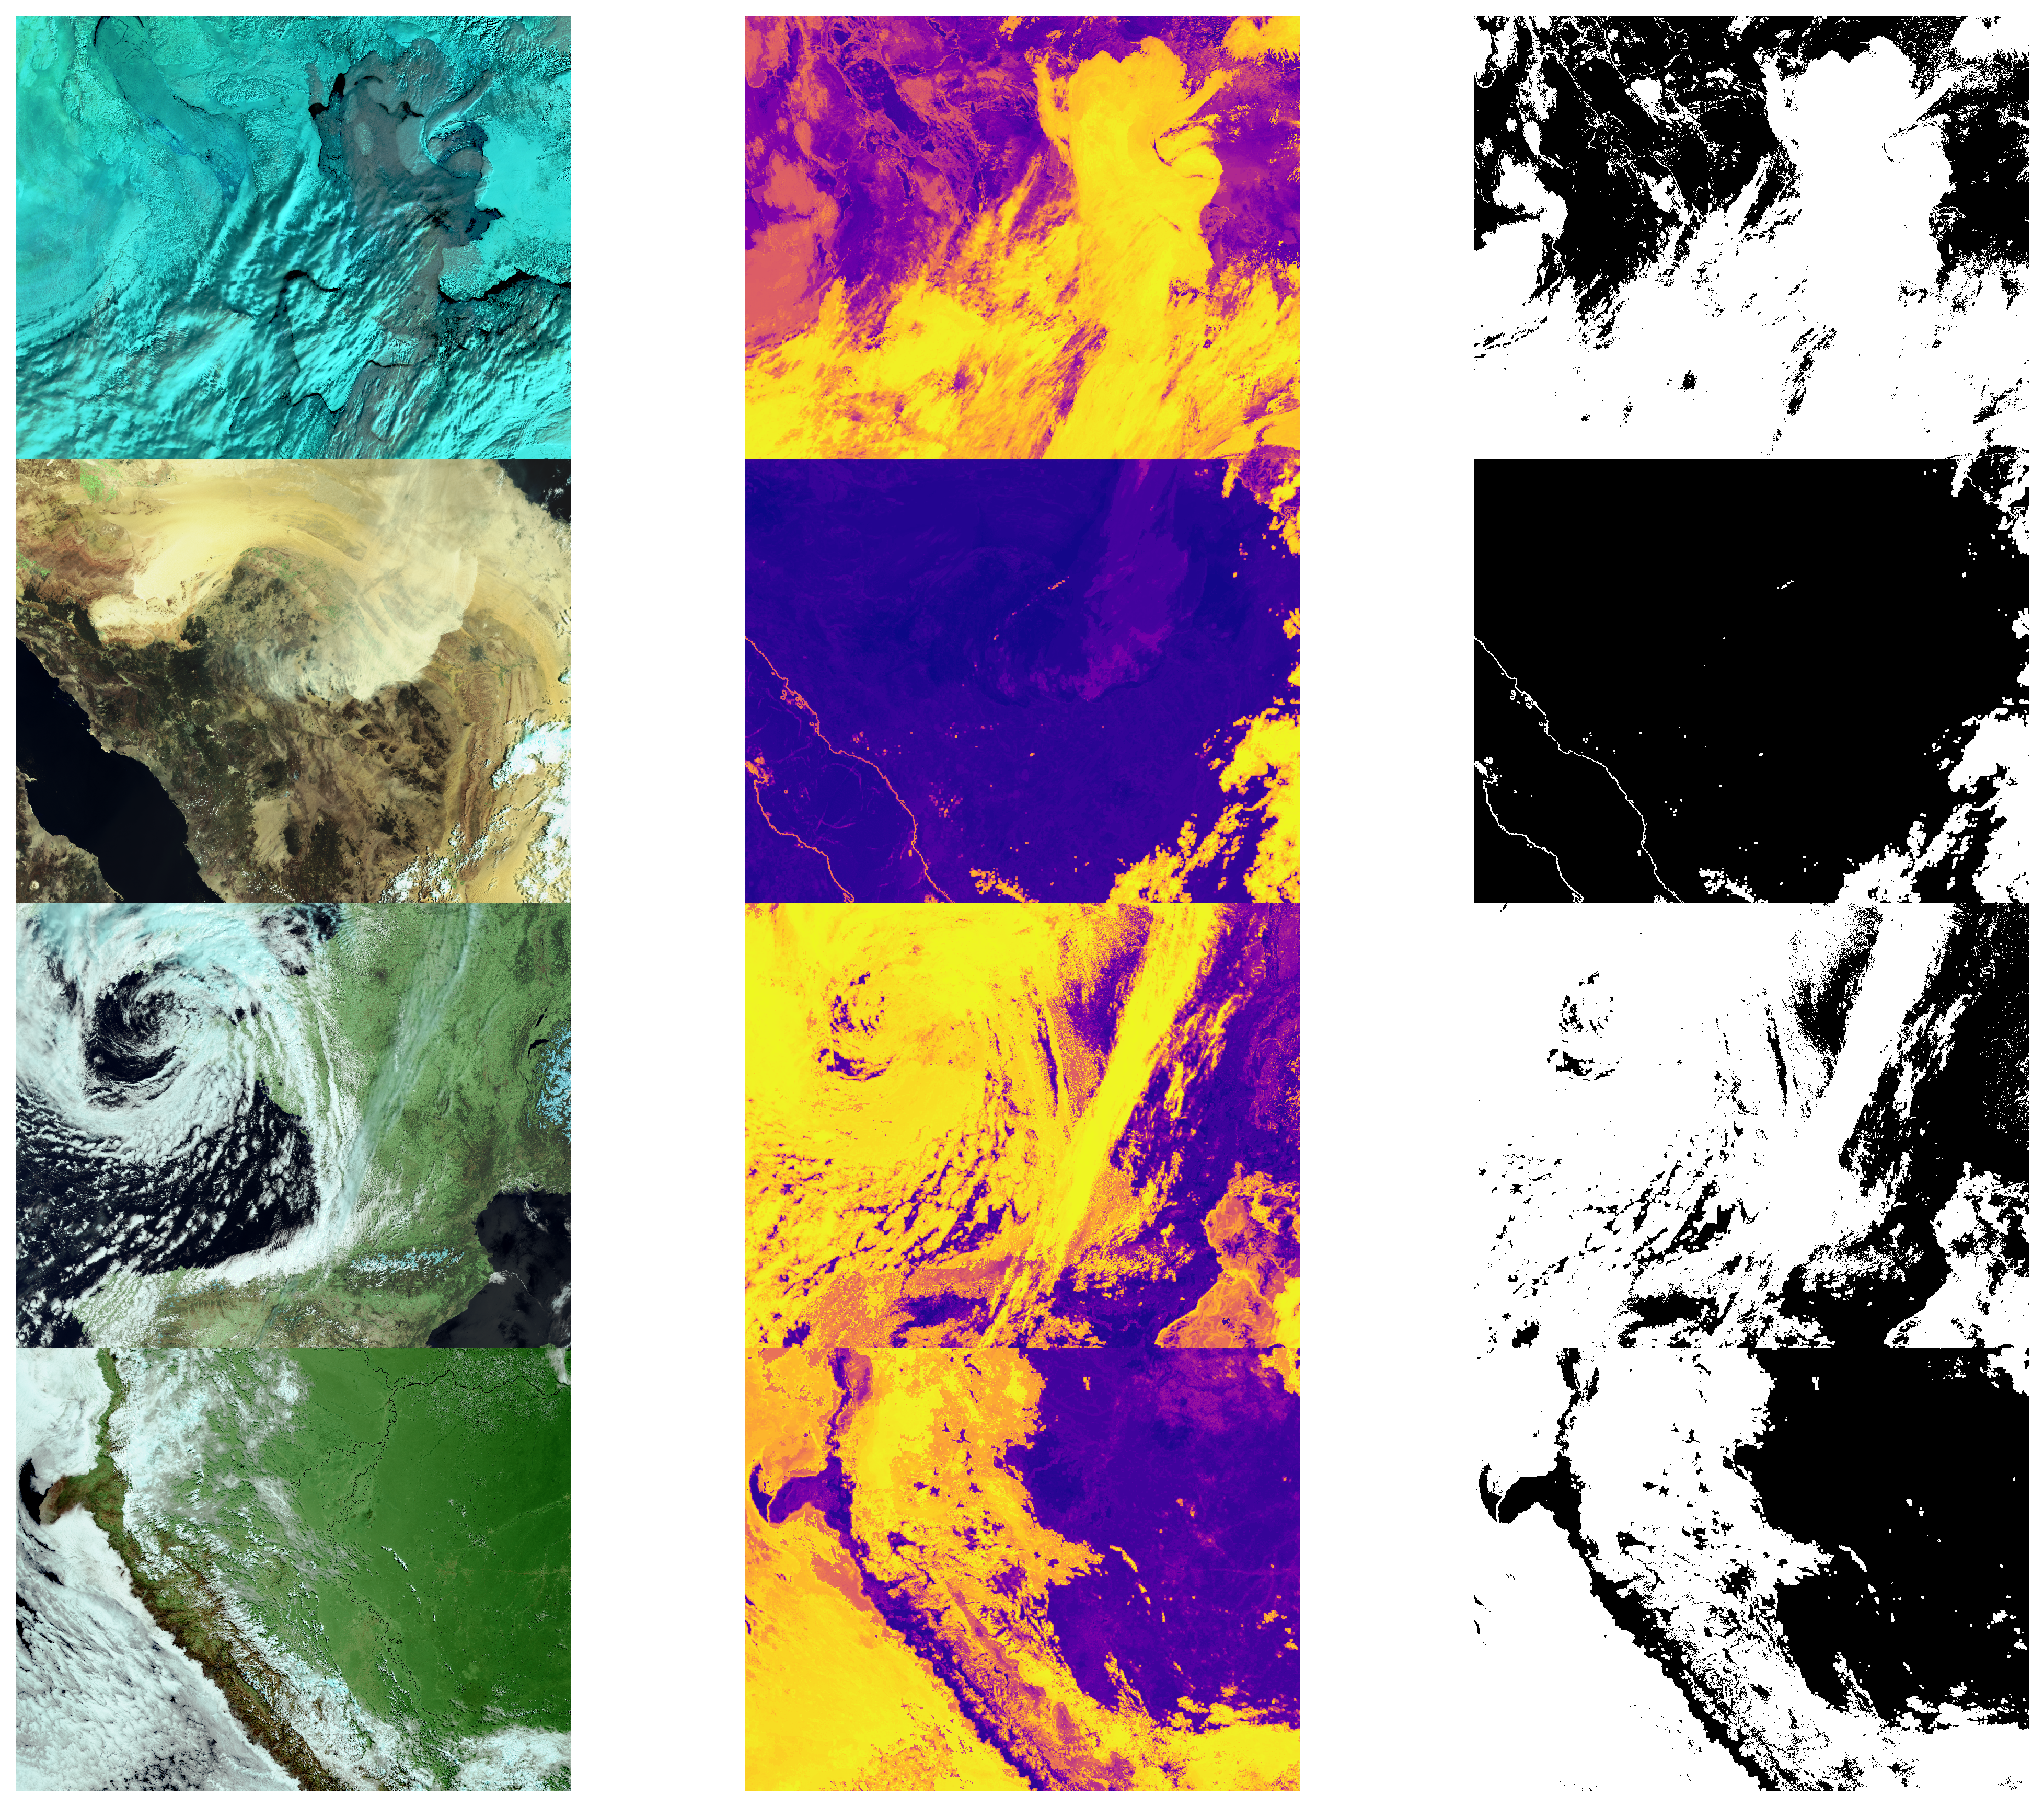
\includegraphics[width=0.5\columnwidth]{images/cloudmask/Figure1_CloudMask_Example.png}
    \caption{Cloud mask example. The left column shows the raw images from the Sentinel-3 satellite while the images on the right column shows the predicted probability that a particular pixel is cloud. }
    \label{fig:cm-example}
\end{figure}


\noindent {\bf Benchmarking Objectives and Metrics:} The scientific objective of the problem is to develop a segmentation model for  classifying the pixels in satellite images. This classification allows determining whether the given pixel belongs to a cloud or to a clear sky. The Bayesian techniques~\cite{merchant:2005} used conventionally can lead to sub-optimal outputs in a number of cases, and hence the scope of the  {\tt cloud-mask} benchmark is to explore whether ML-driven algorithms can outperform the Bayesian techniques. Although various options are there, in its present form, the {\tt cloud-mask} benchmark is set as a supervised learning problem, with cloud images are treated as inputs. However,  like all science cases, the  “true" ground truth (or labels), are never available for this case. Hence, the benchmark uses the Bayesian masks, supplied by the provider of the satellite images, as the ground truth. While this is arguable, we believe that in the absence of any ground truth, this is a valid and perfect choice. However, with Bayesian masks  not always being accurate or not offering a gold-standard for masks,  the resulting model is likely to suffer from learnability issues, which sets the perfect challenge for an ML-driven case. The benchmark can be considered as  both training and inference focused, where the science metric is same as the classification accuracy --- number of pixels classified correctly. The performance metric, can be inference timing and scalability on the training across a number of GPUs. 

\smallskip

\noindent {\bf Data:} The masking can be performed across different satellite imaging modalities. This particular benchmark relies on satellite imagery obtained from the SLSTR sensors equipped as part of the Sentinel-3 satellite. More specifically, the benchmark operates on multi-spectral image data. The overall dataset identified for this benchmark is split into two distinct sets: training set (163~GB) and an inference set (1.7GB). Each dataset inside these sets is made up of two parts: reflectance and brightness temperature. The reflectance is  captured across six channels with the resolution of $2400\times3000$ pixels, and the brightness temperature is captured across three channels with the resolution of $1200\times1500$ pixels. Although the raw satellite images are free to download from the CEDA archive\footnote{\url{https://www.ceda.ac.uk/}}, the curated datasets are available as part of this benchmark, located in object store within the STFC servers. The exact instructions for securing these datasets are outlined in the WG pages. 

\smallskip

\noindent {\bf Reference Implementation:} The current reference implementation is variation of  the U-Net deep neural network \cite{rodenberger-15}, implemented using TensorFlow and Keras, with the support for distributed training using  TensorFlow’s native library, Distributed Mirrored Strategy. The model represents a U-Net network and consists of 39 layers with two million trainable parameters. Further details can be found in~\cite{sciml-bench:2021}.  
